%!TEX program = xelatex

% ==== Part1: 引入latex需要的package,支持不同的需求,如中文、图片 ====
\documentclass[a4paper, 12pt]{article}
% \documentclass[a4paper]{report}
\usepackage[UTF8]{ctex} % 中文latex支持
\usepackage{graphicx} % 引入图片时需要的包
\usepackage{float}    % 插入图片的时候支持`H`这个位置选项
\usepackage{subcaption} % 插入多张图片到一个figure域中
\usepackage{hyperref}   % 插入超链接、TOC支持链接
\usepackage{amsmath,bm} % 一些数序符号、字符
\usepackage{listings}   % 插入代码块
\usepackage{geometry}   % 设置页面四周的边距
% ==== 对引入的package配置 ====
\graphicspath{{images/}} % 配置graphicx这个包:指定图片存储的地方
\hypersetup{ % 设置超链接和url的显示样式
    colorlinks=true,
    linkcolor=blue,
    filecolor=magenta,      
    urlcolor=cyan,
    pdftitle={Overleaf Example},
    pdfpagemode=FullScreen,
    }
\urlstyle{same}

% ==== Part2: latex文档格式配置 ====
\newif\ifchinese % 定义一个条件变量: ifchinese, 作为控制条件编译的开关
\chinesetrue % 条件编译的控制开关,注释掉此部分内容,则对应部分不会被现实
\geometry{a4paper,left=3cm,right=3cm} % 设置左右的页边距


% ==== Part3: latex文档标题部分 ====
\title{加速器配置场景分析}
\author{付杰}
% \author{付杰\thanks{谢谢overleaf提供的LaTex教程}}
\date{\today}


% ==== Part4: latex文档正文部分 ====
\begin{document}
\maketitle
\thispagestyle{empty} % don't use footprint
\newpage

% \begin{abstract} % 摘要
%   \par\textbf{关键字:}LaTex结构、LaTex语法
% \end{abstract}
% \thispagestyle{empty}
% \newpage

\pagenumbering{Roman}
\tableofcontents % 插入目录
\newpage


% \section{条件编译:根据配置的信息,选择编译某一部分的内容}

% \ifchinese
% 这部分是条件编译的内容,必须在\textbf{chinesetrue}判定为真的时候,才会被输出
% \fi


\pagenumbering{arabic}
\setcounter{page}{1}

\newpage 
\section{ACC配置信息写入时的预先设定}%

\begin{enumerate}
  \item L1C作为主处理器负责计算需要下发给加速器的配置信息
  \item L1C计算出的配置信息会被暂存入PPM(Ping Pong Memory)中
  \item PPM内部的配置信息按照(地址,信息)的格式进行存储
  \item PPM内部的配置信息需要具体由DMA或者MCU写入到ACC配置寄存器中
  \item ACC内部的配置寄存器,其地址无法保证连续
\end{enumerate}
  
\newpage
\section{每个ACC都有一套PPM,通过DMA进行配置}%

\begin{itemize}
  \item 工作流:
       \begin{enumerate}
          \item 在这种场景下,L1C计算出每个ACC的配置信息,这些配置信息会被写入到每个ACC的PPM中。L1C跟ACC的AXI Bus采用\textbf{一主多从}的拓扑结构。
          \item 每个ACC内部都有自己的DMA用于从PPM搬运配置信息到ACC内部的寄存器,DMA每次搬运数据都会搬运(地址,信息)这样的而元组数据。
          \item DMA搬运配置信息并且更新ACC配置寄存器的启动,需要由一个信号来控制,这个信号跟ACC以及PPM有关。
          \item ACC内部的配置寄存器组会根据地址来译码选中某一个寄存器,写入的使能信号由DMA给出,将信息写入到该配置寄存器中。
          \item DMA搬运的过程中,每个Cycle有1个ACC配置寄存器可以被更新。
          \item DMA、ACC以及PPM读操作,属于同一个时钟域;L1C跟PPM写属于同一个时钟域。
       \end{enumerate}
  \item 该设计优点:实现上比较简单
  \item 存在的问题:
    \begin{enumerate}
      \item ACC的PPM可能会busy(PPM里的配置信息没有及时被写入到ACC),此时L1C写入到PPM的动作会被阻塞。
      \item PPM利用率不高,这种方式每个ACC的PPM是独享的,某些ACC的PPM可能写不满、另一些ACC的PPM可能不够用,导致了PPM空间的浪费。
      \item L1C需要针对每一个ACC的PPM都有一个AXI Bus连线,需要更复杂的连线以及仲裁结构(L1C不仅需要跟ACC交互,还需要跟其他模块交互)。
    \end{enumerate}
  \item \textbf{适合的工作场景}
    \begin{enumerate}
      \item 对于灵活性要求不高
      \item 允许L1C因为配置PPM而阻塞
    \end{enumerate}
\end{itemize}

系统架构图如图\ref{fig:acc_ppm_dma}所示。
\begin{figure}
  \centering
  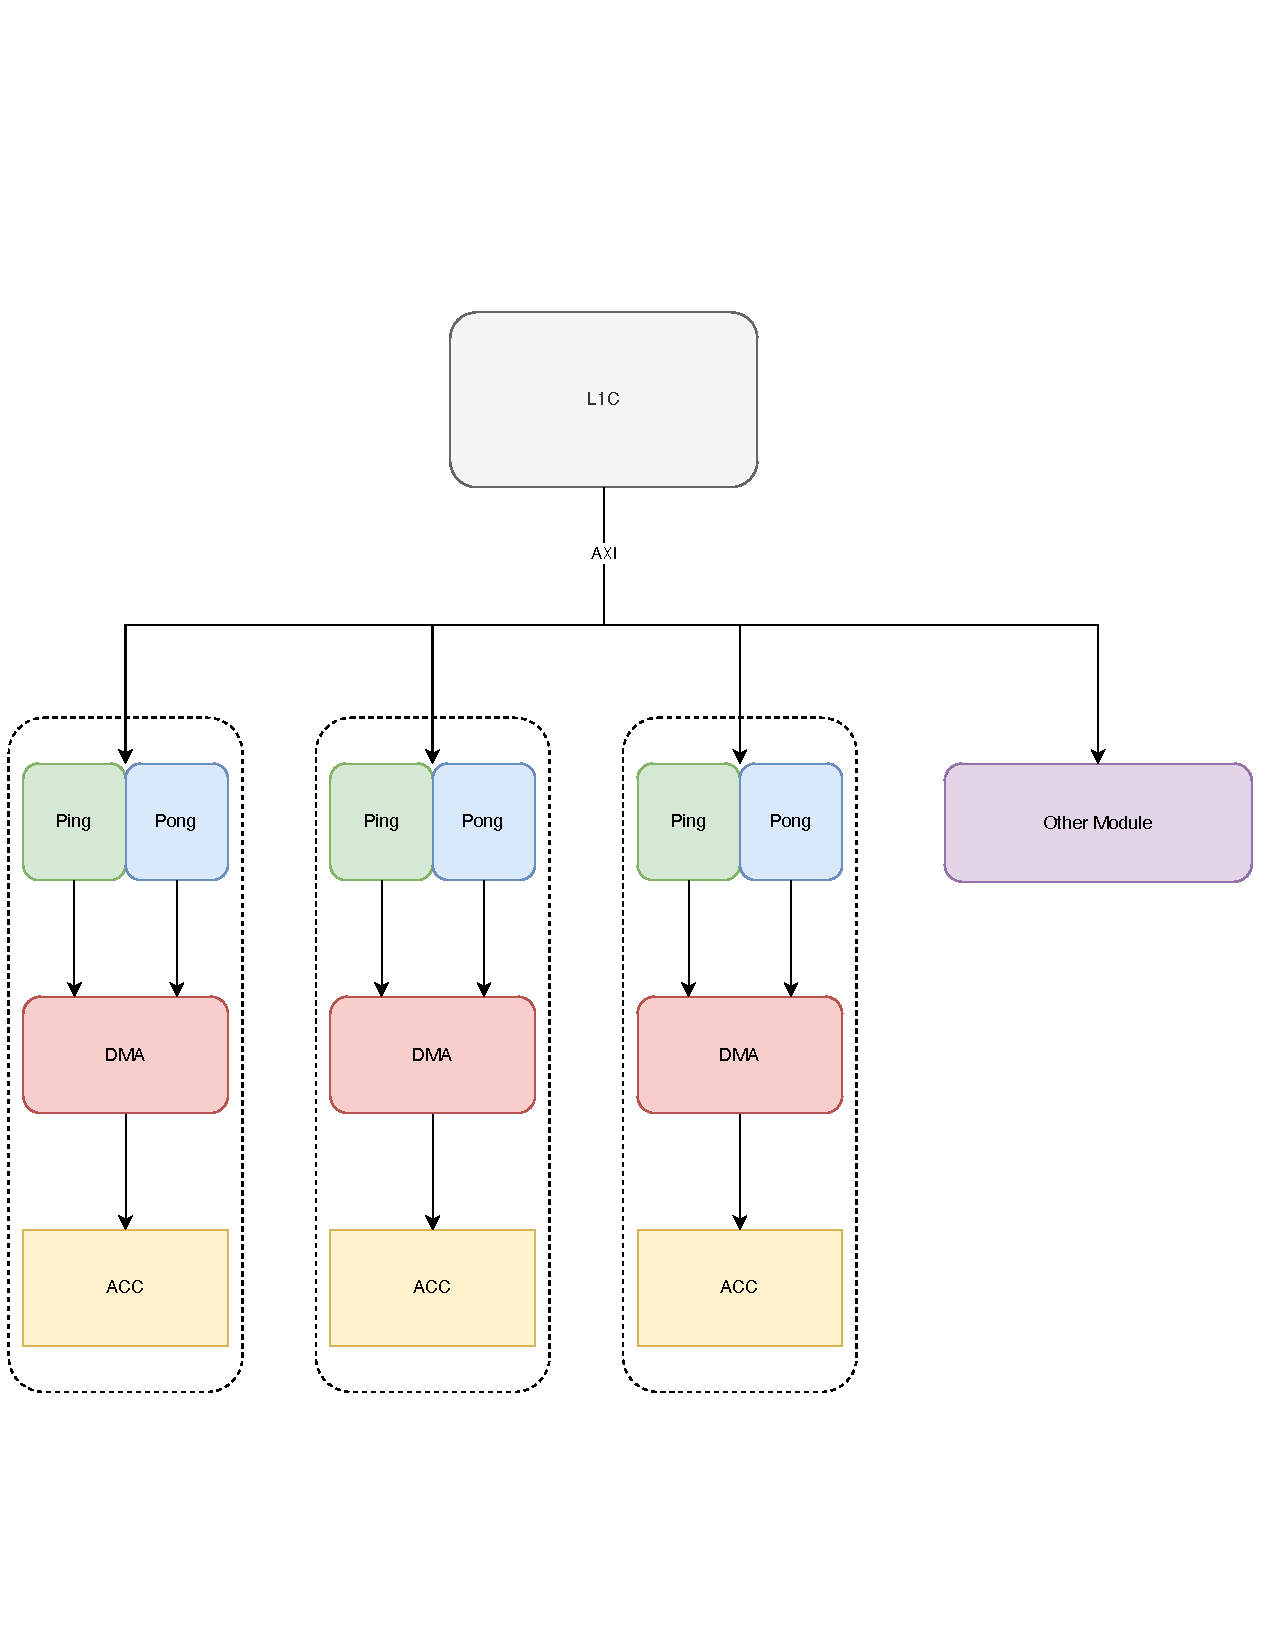
\includegraphics[width=\linewidth]{./images/acc_ppm_dma.pdf}
  \caption{每个ACC都有一套PPM,通过各自的DMA进行配置}
  \label{fig:acc_ppm_dma}
\end{figure}


\newpage 
\section{所有的ACC共享同一块PPM,通过DMA搬运}
\begin{itemize}
  \item 工作流:
    \begin{enumerate}
      \item 所有的ACC不再有自己的PPM,而是共享一块更大的PPM,该PPM可以容纳2N组配置寄存器信息(N为加速器个数)。
      \item 为了支持多个ACC同时从PPM读取配置信息,PPM实际上有多bank构成,进而支持同时读取。
      \item PPM只要有空间,L1C就可以把配置信息写入,此时需要维护一些信息:
        \begin{enumerate}
          \item 这笔配置信息是针对哪个ACC的配置信息。
          \item 修改该ACC对应的配置信息有效队列。
        \end{enumerate}
      \item 每个ACC通过其自己的DMA从统一的PPM搬运配置信息到ACC中。
    \end{enumerate}
  \item 该设计优点:
    \begin{enumerate}
      \item 增加了PPM的利用率以及灵活性。
      \item \textbf{简化了L1C写入到PPM的过程},L1C不用跟每个ACC都有AXI总线连接,避免了总线busy的情况。
    \end{enumerate}
  \item 存在的问题:
    \begin{enumerate}
      \item PPM被L1C写入的时候,需要维护额外的与ACC的映射关系。
      \item PPM需要支持多端口读,且PPM跟每个ACC都需要通过AXI总线连接。
    \end{enumerate}
  \item \textbf{使用的场景}:
    \begin{enumerate}
      \item 加速器内部寄存器需要配置的情况比较简单,简单地就能判断是否需要发起对加速器的配置更新,此时通过DMA直接进行配置
      \item 某些加速器其内部PPM不够用导致加速器性能出现瓶颈、而其余加速器内部PPM空闲
    \end{enumerate}
\end{itemize}

系统架构图如图\ref{fig:acc_dma}所示。
\begin{figure}
  \centering
  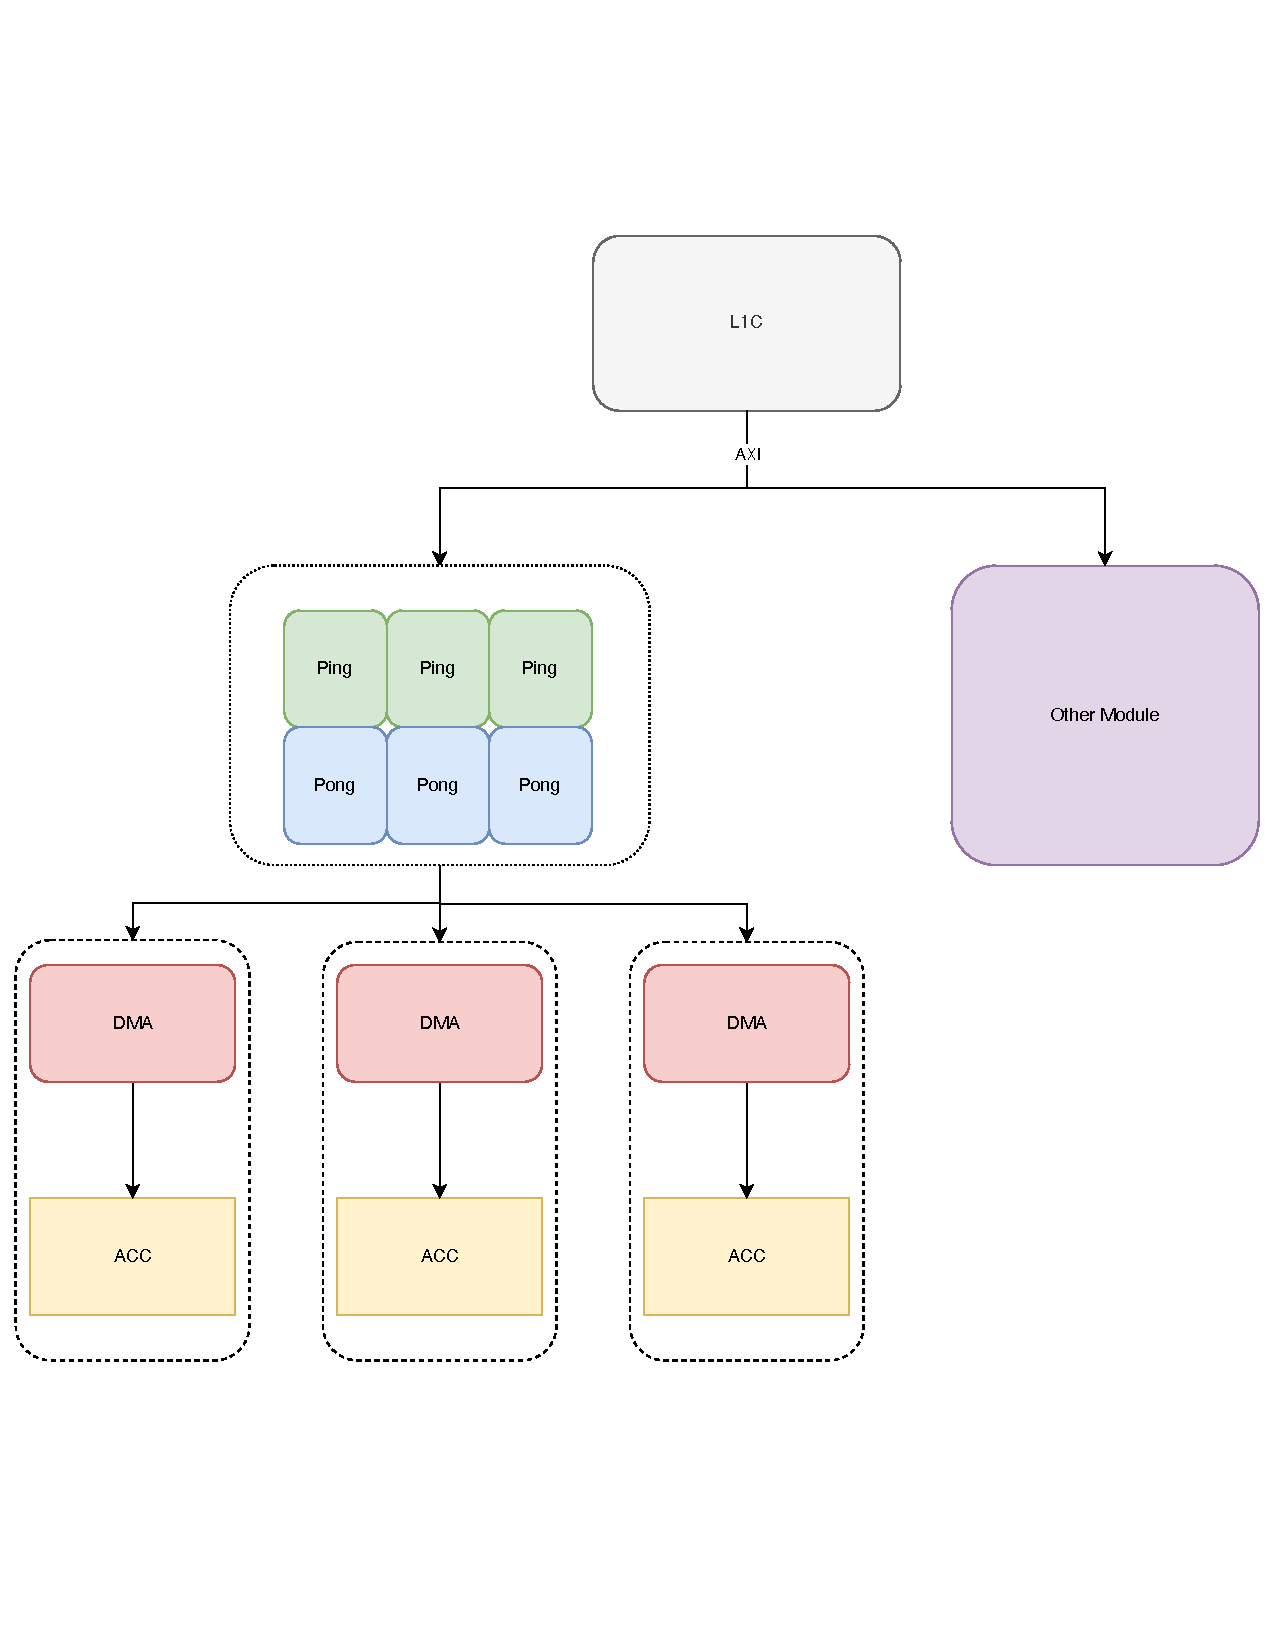
\includegraphics[width=\linewidth]{./images/acc_dma.pdf}
  \caption{每个ACC共享一套PPM,通过各自的DMA进行配置}
  \label{fig:acc_dma}
\end{figure}

\newpage 
\section{所有的ACC共享同一块PPM,通过MCU搬运}%
\begin{itemize}
  \item 工作流:
    \begin{enumerate}
      \item 每个加速器内部没有DMA,数据的搬运通过MCU从PPM搬运到每个ACC中
      \item 满足ACC配置的条件之后,可以发起一个中断,触发MCU进入到配置ACC的中断处理程序中去
      \item MCU每一次配置ACC,都可以由程序发起,程序可以指定:
        \begin{enumerate}
          \item PPM读取地址的base address
          \item PPM读取的配置信息的数量
          \item 需要配置的ACC
        \end{enumerate}
      \item 如果配置的过程被中断了,可以很好地在中断处理结束之后继续之前的配置流程
    \end{enumerate}
  \item 该设计优点:
    \begin{enumerate}
      \item 灵活性最高,配置信息写入到ACC的过程甚至可以由软件进行控制
      \item MCU跟ACC之间的AXI总线不需要仲裁结构,因为MCU一次只能配置一个ACC
      \item PPM只用提供一套读端口供MCU读取即可
    \end{enumerate}
  \item 存在的问题
    \begin{enumerate}
      \item MCU一次只能下发配置信息到一个ACC
      \item 单笔配置信息包含两个动作load, store,对比与DMA来说,效率不高
      \item MCU需要运行其他任务,ACC的配置动作可能会被interrupt
    \end{enumerate}
  \item \textbf{适合的工作场景}:
    \begin{enumerate}
      \item L1C需要处理除ACC配置之外的其他很多事务,L1C计算出的配置信息需要有简单的存储方式进行暂存,从而解放L1C去做其他的事务
      \item 加速器需要配置信息更新的条件比较复杂,无法简单确定什么时候加速器的配置信息需要更新
      \item 加速器需要配置的寄存器数量不是很多,\textit{若一个加速器的配置就需要占用MCU很长的时间,导致其他加速器配置暂停,就不适用}
      \item 加速器内部不包含DMA控制器的情况
    \end{enumerate}
\end{itemize}
  
系统架构图如图\ref{fig:acc_mcu}所示。
\begin{figure}
  \centering
  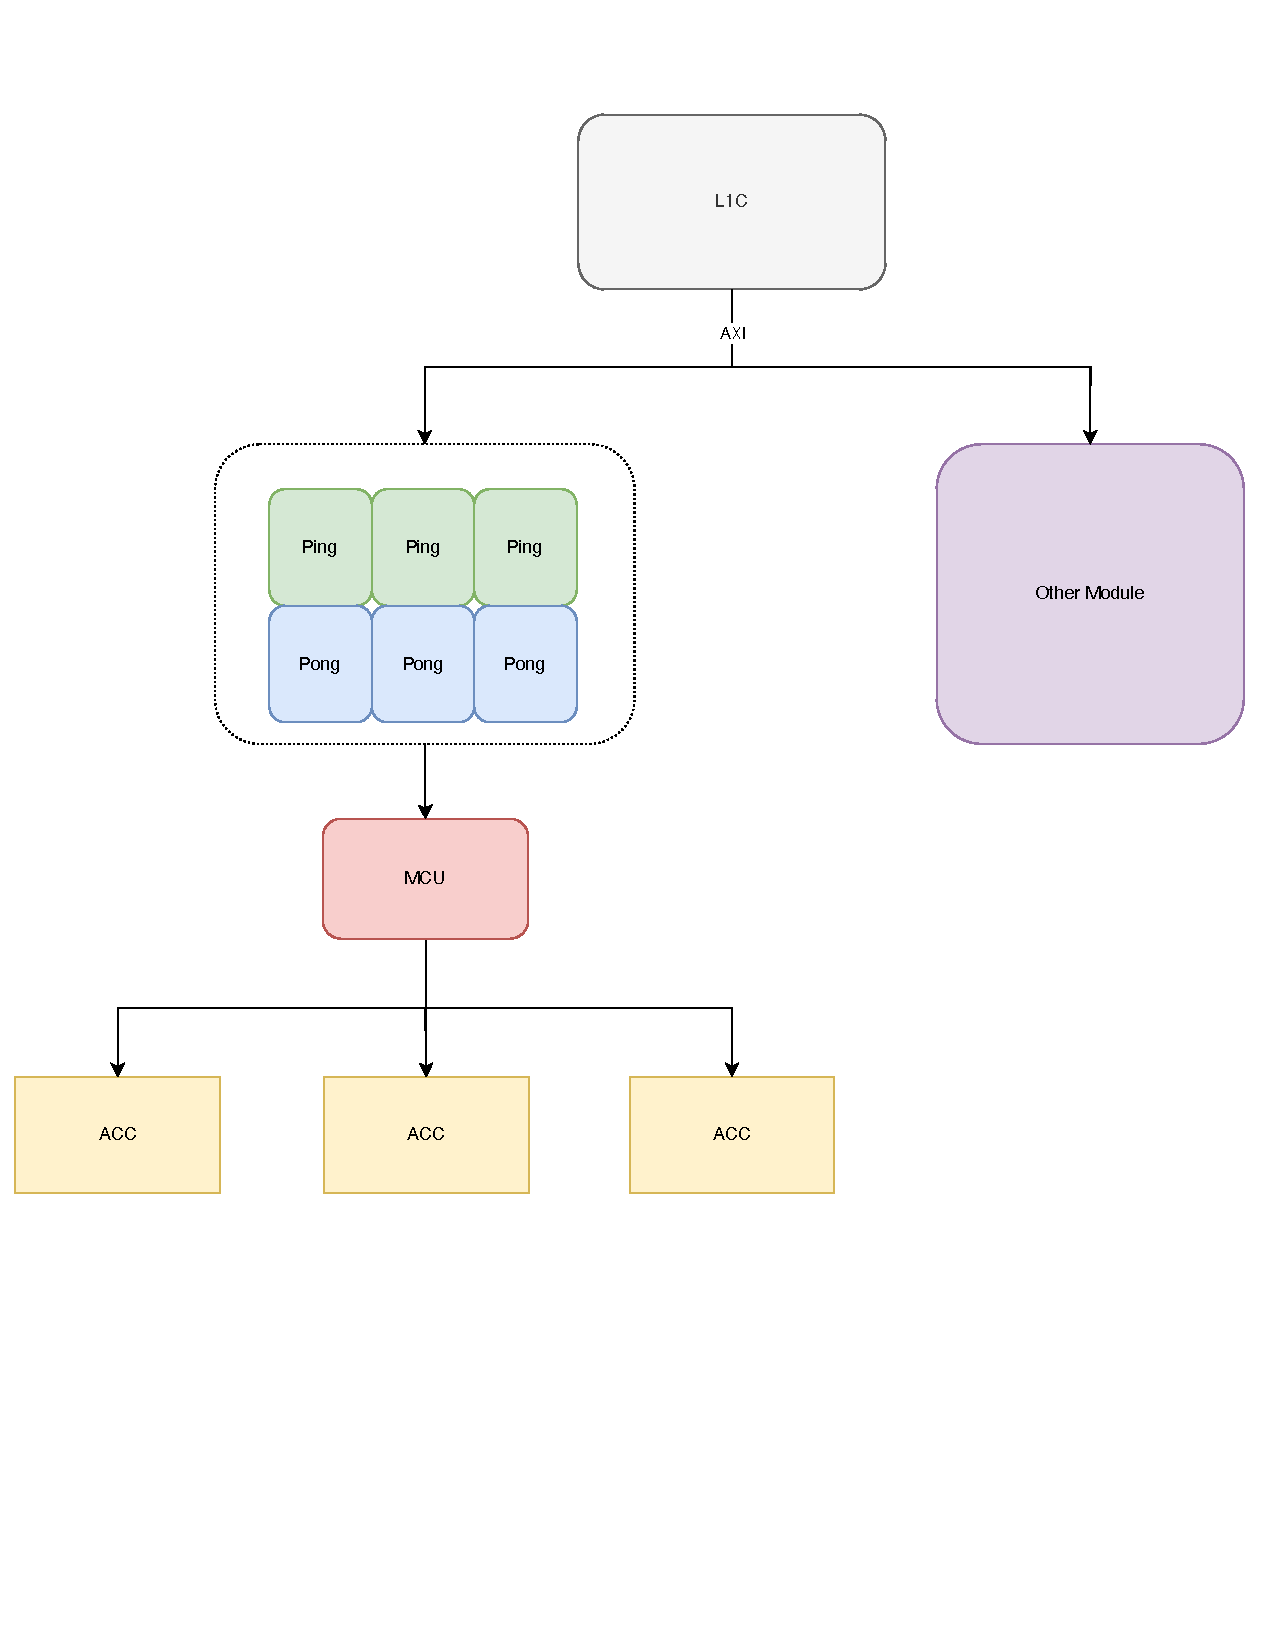
\includegraphics[width=\linewidth]{./images/acc_mcu.pdf}
  \caption{每个ACC共享一套PPM,通过MCU进行配置}
  \label{fig:acc_mcu}
\end{figure}

\newpage
\section{一些想问的问题}%
\begin{itemize}
  \item \textbf{问题一:}
        加速器是否需要等到所有配置信息都更新完毕了再开始计算?
        \begin{enumerate}
          \item 在配置加速器配置寄存器的时候,加速器是不是不能开始计算?
          \item 如果是这样的话,那么加速器本身是否需要一个信号来告知
                它配置信息已经更新完毕了。
          \item 加速器内部是否有一个\textbf{flag}寄存器,
                用来表示寄存器配置是否完成?
        \end{enumerate}
  \item \textbf{问题二:}什么时候更新ACC的配置寄存器信息?
        \begin{enumerate}
          \item L1C计算出的一组配置信息写入到PPM的时候,就需要更新ACC的配置寄存器嘛?此时L1C是否会拉高相应的信号?
          \item PPM内部是否只能同时存在一组配置信息,这样每次更新PPM之后都表示需要更新ACC配置寄存器了。
          \item 配置信息的更新,应该需要加速器把当前正在进行的计算完毕再更新,那么计算器是否需要给出一个信号(中断)来告诉MCU或者DMA自己当前计算完毕了,可以更新配置寄存器?
        \end{enumerate}
  \item \textbf{问题三:}如何界定L1C一组配置信息的边界?\\假如L1C有两组给同一个ACC的配置信息,那么这两组配置信息的边界,是怎么给出的?
  \item \textbf{问题四:}ACC的配置寄存器跟ACC需要计算的数据源是什么关系?
        \begin{enumerate}
          \item 其配置信息是由L1C计算得出的,那么需要计算的数据由什么给出?
          \item 配置信息的更新跟数据源的更新,是否需要同步?
          \item 计算完多少组数据之后,需要更新配置寄存器?
        \end{enumerate}
  \item \textbf{问题五:}假设PPM的可以容纳M条配置信息,但是L1C只写入了N条配置信息$N < M$
    \begin{enumerate}
      \item 那么在写入配置信息的时候,如何处置PPM里无效的那些配置信息?
      \item DMA搬运的时候,会只搬运有效的配置信息的部分然后就结束任务吗?
    \end{enumerate}
\end{itemize}

% \newpage
% \bibliography{ref} % 参考文献源,存储所有的参考文献
% \bibliographystyle{IEEEtran} % latex饮用参考文献时的格式

\end{document}


